% !TeX root = ../thesis.tex
% TH-CH03-WRITE-V1: stage 3 draft; not compiled or frozen.
\chapter{面向灵巧手操作的抓取候选生成与专家示教构建}
\label{chap:grasp_demonstrations}

\section{抓取任务定义与总体流程}
\label{sec:grasp_task_pipeline}

第二章建立了机器人执行与触觉观测的仿真基础，但具有可控模型并不意味着能够直接生成有效操作轨迹。面对不同形状和摆放状态的物体，系统既要寻找手部可形成接触的构型，也要使该构型满足机械臂运动约束，并在实际动力学推进后保持物体。因此，本章从候选生成、机器人约束筛选、轨迹执行和质量验收四个层次展开：先寻找可抓取构型，再检验机械臂能否到达、操作能否执行以及所得轨迹是否满足示教要求。

抓取输入包括物体标识、表面采样及法向、初始位姿与任务条件。候选以物体坐标系下的手部平移、旋转和六维驱动比例表示，可记为
\begin{equation}
 \mathcal G=(\boldsymbol t_{oh},\boldsymbol R_{oh},\boldsymbol f,\mathcal C,\boldsymbol m),
 \qquad \boldsymbol f\in[0,1]^6,
 \label{eq:ch03_candidate}
\end{equation}
其中，$\boldsymbol t_{oh}\in\mathbb R^3$和$\boldsymbol R_{oh}\in SO(3)$描述物体坐标系下的手部目标，$\mathcal C$存储接触点、法向及距离，$\boldsymbol m$为候选质量和来源指标。驱动比例需进一步转换为具体执行器的控制范围，不等于十二个手部关节的独立角度。候选合同检查维度、旋转合法性和比例范围，这些检查只能保证表达有效，不能证明实际接触已经成立。

\begin{figure}[htbp]
  \centering
  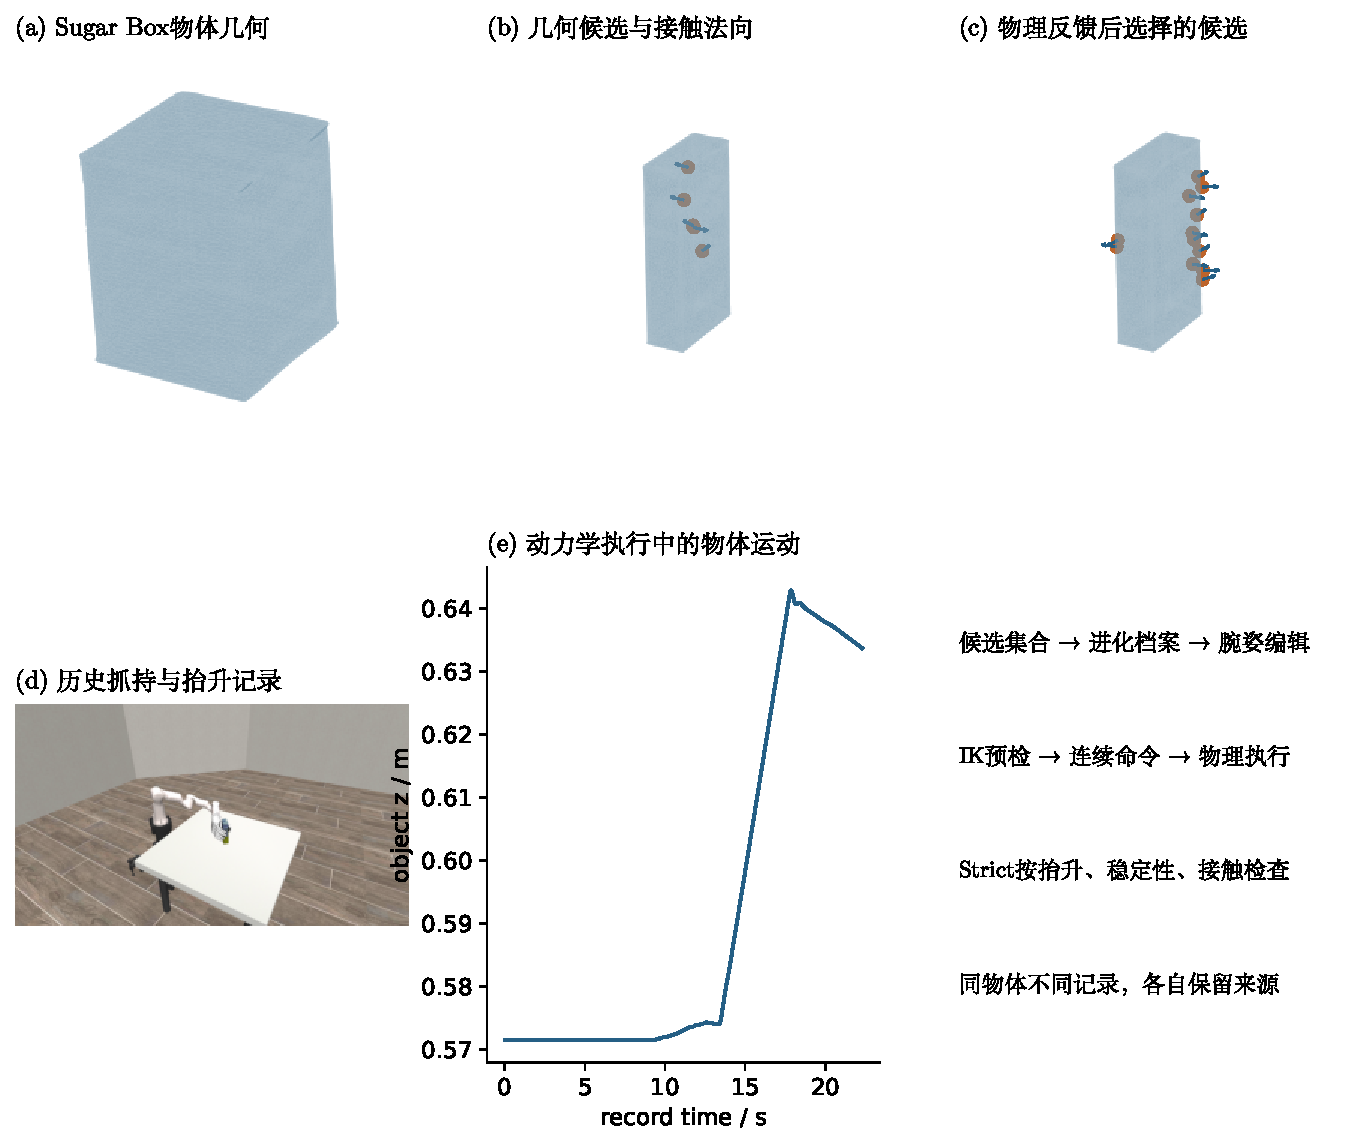
\includegraphics[width=0.97\textwidth]{figures/annotation_R2/grasp_evidence_pipeline.pdf}
  \caption{Sugar Box同物体案例的候选几何、执行反馈与示教构建证据}
 \label{fig:ch03_overall_pipeline}
\end{figure}

图\ref{fig:ch03_overall_pipeline}以Sugar Box贯穿候选几何与执行反馈：物体表面和保存的接触候选为几何评价提供输入，进化档案补充物理反馈，腕姿扩展与IK筛选再连接机械臂目标，连续命令进入实际执行与Strict回放。各画面保留原始记录身份，用于说明同一物体上的各环节，而非将不同候选拼成同一条优化轨迹。机器人约束筛选将对象相对目标转换为世界坐标下的机械臂末端目标，轨迹执行再连接接近、闭合、保持和后续操作。只有经过执行，才能获得状态、接触和物体运动等反馈；Strict质量验收进一步检查尾段稳定性。Lift提供抓持和抬升的基本案例，搬移与堆叠可在抓持前缀上构造任务后缀，推动和装配则需要额外的接触或姿态控制。五类任务共享示教数据合同，但不共享完全相同的物理执行逻辑。本章重点讨论示教如何形成，记录关联、数据转换与全量质量审计留在第四章。

\section{多来源抓取候选生成}
\label{sec:grasp_candidate_generation}

欠驱动手的关节并非独立受控，直接优化全部关节角可能偏离实际可执行构型。本文以六个驱动比例为手部参数，利用仿真采样拟合的皮肤点轨迹代理连接驱动与接触几何。该代理用于可微评价，其范围受采样和模型版本限制，最终行为仍需物理反馈检验。

GraspQP通过可微抓取质量评价支持候选优化\cite{zurbrugg2025graspqp}。本文调用其官方指标工厂，结合物体表面点、法向和手部代理构造接触评价。优化变量包括三维平移、六维旋转参数及六个驱动比例的logit，驱动比例通过sigmoid限制在有效区间。旋转参数在评价时恢复为旋转矩阵，从而避免直接优化九个任意矩阵元素。物体采样和手部皮肤点变换到同一坐标下后，程序按手指接触点组计算到物体的距离，并以软权重构造接触位置和法向。由此形成的接触集合用于官方质量指标计算，而不是把最近点距离本身当作力闭合证明。

单独优化抓取指标可能得到难以执行的构型，因此目标还加入接触距离、穿透、桌面距离、平移漂移和驱动耦合约束。接触距离项鼓励手部采样点接近物体；穿透和桌面项限制明显不合理的几何关系；漂移项抑制手部偏离初始种子过远；驱动耦合项约束部分手指比例的离散程度。各项具有不同归一化尺度与权重，其数值意义应结合实际实现解释。表\ref{tab:ch03_candidate_parameters}列出变量和约束的职责。这一适配使官方抓取指标能够作用于六驱动手的构型变量，后续仿真反馈进一步评价加载后的接触保持。

\begin{table}[htbp]
 \centering\small
 \caption{候选优化参数及约束的实际作用}
 \label{tab:ch03_candidate_parameters}
 \begin{tabular}{p{0.20\textwidth}p{0.25\textwidth}p{0.41\textwidth}}
 \hline
 项目 & 表达或输入 & 作用与边界\\
 \hline
 手部平移与旋转 & 三维平移、六维旋转参数 & 搜索对象相对手部位姿，输出合法旋转矩阵\\
 手部驱动 & 六维比例logit & 经sigmoid形成执行器比例，不独立控制全部关节\\
 接触几何 & 表面点、法向及距离 & 连接手部代理与物体几何评价\\
 官方抓取指标 & 接触集合与摩擦设置 & 提供几何抓取质量，不代替机器人执行\\
 附加几何约束 & 接触、穿透、桌面距离 & 排除部分明显不合理的候选\\
 漂移与驱动约束 & 种子平移及驱动比例 & 限制局部搜索偏移和驱动分散\\
 \hline
 \end{tabular}
\end{table}

几何候选进入DexEvolve-style细化阶段后，评价对象从接触构型扩展到执行行为。DexEvolve原研究采用进化优化获得多样且稳健的灵巧抓取\cite{zurbrugg2026dexevolve}，本文保留候选群体、变异、交叉和档案管理的组织思想，并针对六驱动手及现有仿真执行接口作适配。平移、旋转和驱动比例分别施加扰动，驱动变化限制在有效范围内；交叉则组合不同候选的位姿与手部配置。候选在执行前还可进行接触修正和去穿透处理，使搜索不仅依赖最初的几何种子。

物理反馈通过实际执行候选获得接触保持、物体相对漂移和扰动响应等指标，必要时使用MJWarp后端评价寿命相关目标。几何质量较高的构型仍可能在接近时偏离物体，或在加载后因接触方向不合适而失稳，因而物理反馈不能由静态接触分数完全替代。进化档案利用候选距离、新颖性及局部密度等信息保留不同构型，避免全部预算集中到近乎重复的局部解。档案按平移、旋转和驱动比例构成的嵌入计算候选距离；新候选若与最近档案项的距离小于新颖性阈值，仅在适应度更高时替换该项，否则作为新构型加入。父代选择再以局部密度修正适应度，减少拥挤邻域反复占用搜索预算；最终按适应度整理候选，供后续腕姿与机器人约束筛选。

\begin{figure}[htbp]
  \centering
  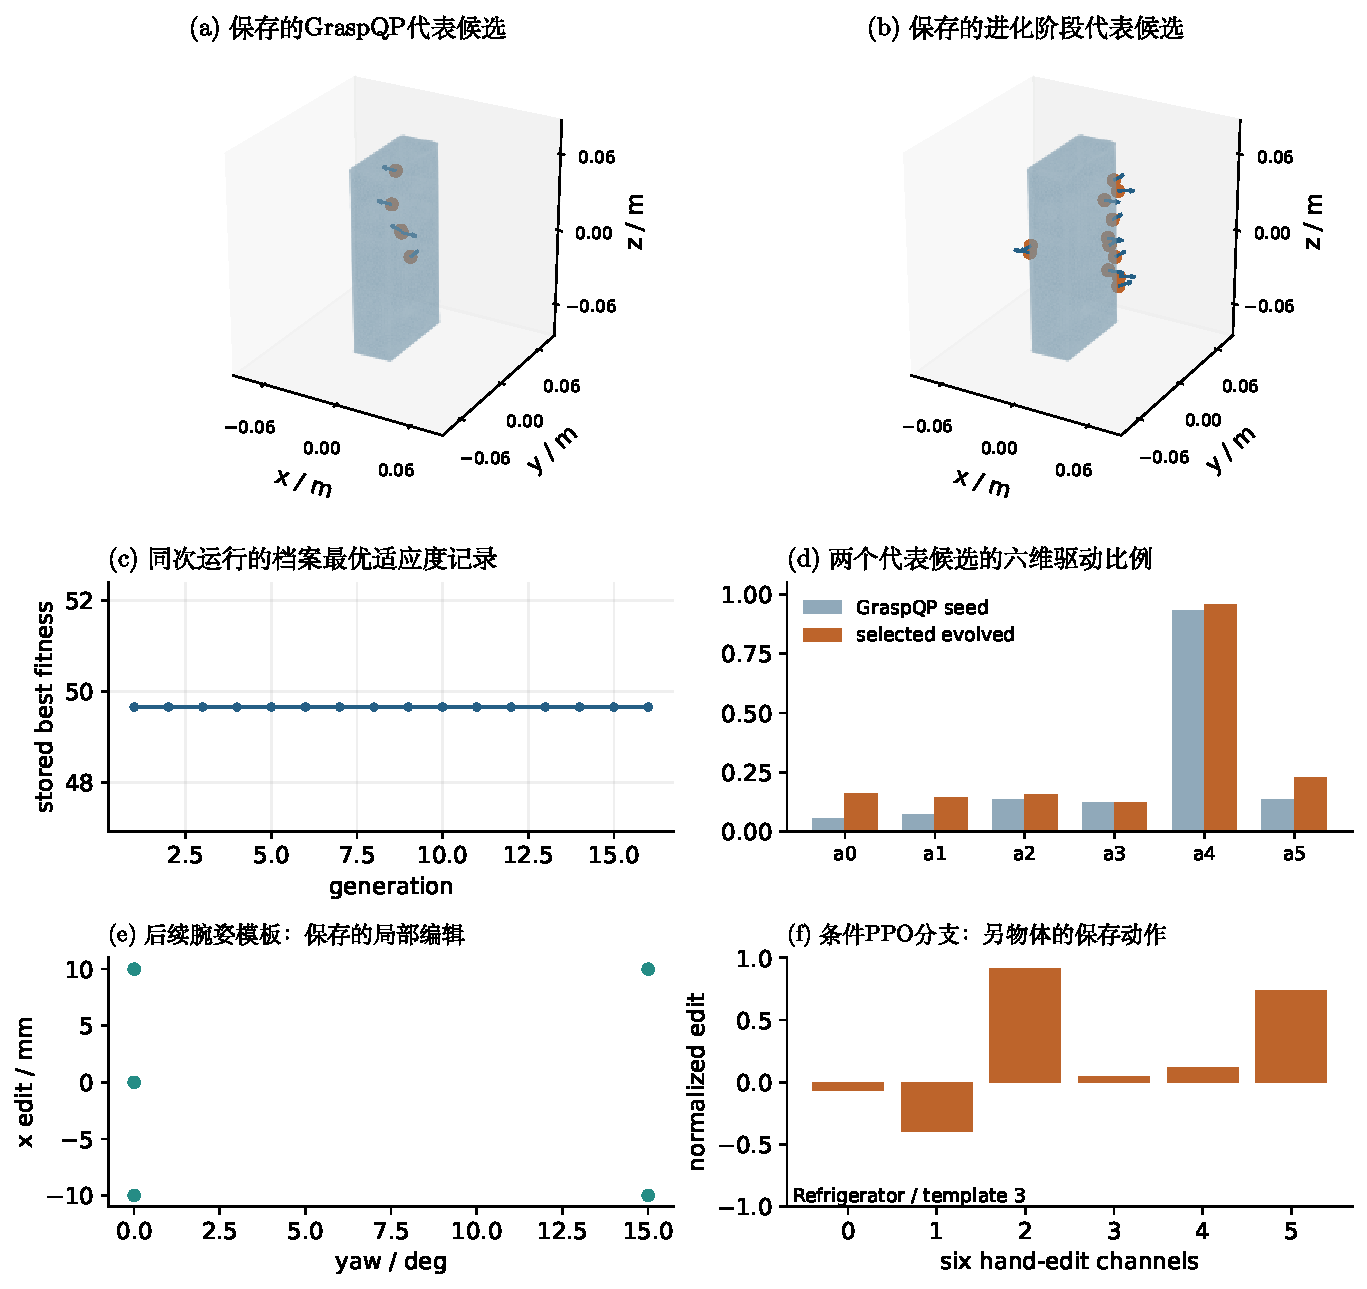
\includegraphics[width=0.97\textwidth]{figures/annotation_R2/candidate_geometry_feedback.pdf}
  \caption{代表候选、进化档案、腕姿模板与条件PPO分支的保存记录}
 \label{fig:ch03_candidate_sources}
\end{figure}

腕部姿态格点扩展（Wrist Lattice）用于搜索源候选附近更容易被机械臂到达的手腕位姿。它在源候选附近改变腕部平移和朝向，再以机器人逆运动学残差排序，保留可进一步执行的模板。当前默认集合包含39个格点，平移基本尺度为0.01~m，旋转基本尺度为$15^\circ$，并包含若干倍尺度的单轴旋转以及平移、旋转耦合编辑。该邻域保留源抓取附近的接触构型，同时为机械臂提供不同的腕部目标。39个格点是同一源候选的搜索编辑，预算按被评价的候选计量；搜索范围由所设平移与旋转尺度限定。

统一生成预算配置当前采用64个种子、150步GraspQP优化并执行12个候选；进化阶段使用24个初始个体、每代12个子代、16代，名义候选评价次数为216，随后向腕部扩展提供最多6个档案候选。这些是当前入口默认预算；历史批次及缓存复用的实际代价需另行区分。

图\ref{fig:ch03_candidate_sources}展示同次运行保存的几何候选、进化代表候选及档案最优适应度；接触点与法向直接来自候选文件，六维驱动比例反映不同抓持配置。MJWarp PPO仅作为条件性补充，在格点阶段未解决且仍有可用模板时进行模板选择与手部驱动编辑，图中另以Refrigerator记录展示该分支保存的模板选择与六维手部编辑，和Sugar Box的几何、进化与腕姿记录分别标识。历史Top100路由中存在2条RL\_SUCCESS记录，但这并不构成强化学习优于其他模块的消融证据。整体而言，可微指标提供几何方向，进化反馈检验物理行为，格点扩展处理机器人可达性，后续编辑尝试解决局部未完成案例。各模块依赖不同输入和预算，应分别说明作用，不能混合命名为一个新的原创抓取优化算法。

\section{基于可达性约束的抓取筛选}
\label{sec:grasp_reachability}

对象相对抓取只有在转换到机器人末端目标后，才能评价机械臂是否能够执行。设物体世界位姿为$(\boldsymbol R_{wo},\boldsymbol p_{wo})$，候选定义的手部目标为$(\boldsymbol R_{oh},\boldsymbol t_{oh})$，则目标手部姿态与末端姿态满足
\begin{equation}
 \begin{aligned}
 \boldsymbol p_{wh}&=\boldsymbol p_{wo}+\boldsymbol R_{wo}\boldsymbol t_{oh},\\
 \boldsymbol R_{wh}&=\boldsymbol R_{wo}\boldsymbol R_{oh},\qquad
 \boldsymbol R_{we}=\boldsymbol R_{wh}\boldsymbol R_{eh}^{\mathsf T}.
 \end{aligned}
 \label{eq:ch03_target_transform}
\end{equation}
其中，$\boldsymbol R_{eh}$为手部安装相对旋转，$w,o,h,e$分别表示世界、物体、候选手部参考与末端坐标。位置量单位为m，旋转无量纲。这里采用执行器接口中实际使用的安装参考，不能把STL局部原点任意替换为另一个掌心点后仍沿用同一公式。若缺少安装补偿，即使目标手部方向在几何上正确，机械臂实际跟踪方向也可能与之不同。

预抓取目标沿候选手部局部方向向外退让，当前默认距离为0.09~m；抓取目标则对应候选位置本身。筛选器按预抓取、抓取的顺序调用实际机械臂IK，在前一个求解结果上继续处理后一个目标。它同时记录位置残差、旋转残差与末端行程，用于区别几何合理但机器人难以到达的候选。检查过程中会保存并恢复环境状态、执行器控制量以及控制器历史目标，避免静态候选排序直接改变后续真正执行的起点。

当前排序器采用如下评分：
\begin{equation}
 S_{\mathrm{reach}}=20e_p^{\max}+0.6e_R^{\max}+0.08\ell,
 \label{eq:ch03_reachability_score}
\end{equation}
其中，$e_p^{\max}$和$e_R^{\max}$分别为两个目标上的最大位置与旋转残差，$\ell$为相应末端行程。三个系数是代码中的数值权重，用于产生排序，而非经过物理标定的统一距离单位。评分较小表示在该初值和求解配置下更易到达，不表示对应抓持必定稳定。静态排序还临时放宽目标速度约束，使残差更接近求解可达性的检查；真正执行时仍使用相应速度限制和平滑，不能将两条路径的跟踪结果视为相同。

模板构建依据执行配置保留位置误差不超过0.025~m、旋转误差不超过0.22~rad的候选。这两个容差属于当前生成执行层的筛选设置，不是第二章控制器内部更严格的迭代终止容差。满足筛选容差后，还需要根据腕部编辑幅度、源轨迹动态跟踪误差和候选评分确定执行顺序。这样既考虑静态残差，也保留对原有接触构型的偏好，避免搜索一开始就使用偏移很大的变体。

\begin{figure}[htbp]
  \centering
  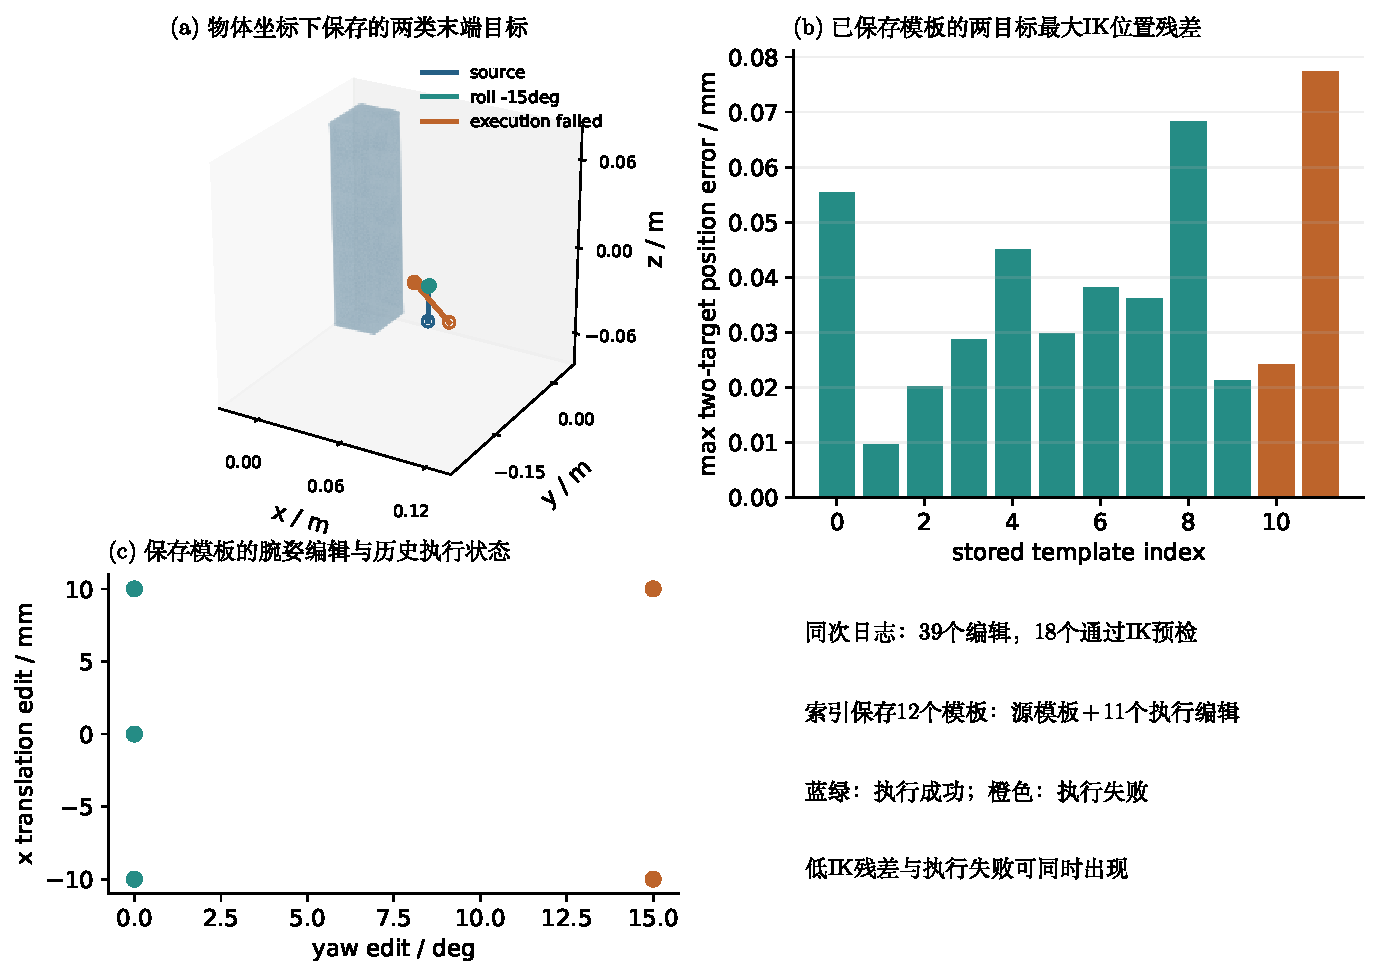
\includegraphics[width=0.97\textwidth]{figures/annotation_R2/wrist_recorded_targets.pdf}
  \caption{腕姿模板的保存目标、预检残差与历史执行结果}
 \label{fig:ch03_reachability}
\end{figure}

图\ref{fig:ch03_reachability}所示预检的作用范围需要明确：已核验实现主要覆盖预抓取与抓取两个目标，并没有据此证明完整Lift轨迹的每个路点都通过连续碰撞认证。两个端点均可达时，中间路径仍可能靠近桌面或改变IK分支；静态残差较小时，动态跟踪也可能因速度限制而产生更大误差。因此，筛选结果只决定候选是否值得进入执行，后续阶段仍需读取真实状态和接触结果，不能把它称为通用连续无碰撞规划器。

不同约束在流程中承担不同职责。候选优化中的桌面距离惩罚限制明显不合理的初始几何，任务迁移中的保守下降高度控制局部接近，执行过程监测接触和目标误差，Strict则对尾部桌面接触及稳定性作最终判断。这些机制相互补充，但不应合并为一个未经实现的全局碰撞约束。对失败也应保留层次：无有效候选、静态IK残差过大、动态接近偏差、闭合后缺少对向接触和抬升失稳对应不同问题。只有明确失败发生在哪一层，才能避免把所有失败归因于抓取几何质量。

局部搜索还受预算限制。模板构建对可执行候选排序后，只运行有限数量的完整尝试，并可优先复用已有参考。这有助于控制批量生成代价，但意味着最终保留下来的模板不等于全部可达候选，也不构成对整个抓取空间的穷举。本文将这种筛选视为面向具体机器人和源候选的约束连接环节，其有效范围由后续实际执行与验收结果共同确定。

图\ref{fig:ch03_reachability}将腕姿编辑与已保存的预检结果对应。同次日志登记39个编辑中18个通过预抓取及抓取两目标检查，模板索引保存其中12个执行或复用模板。图中的残差是两目标误差的最大值；橙色模板虽然预检残差较小，实际执行仍失败。这说明腕姿可达性只解决目标求解条件，后续接触保持仍需通过物理执行检查。被预检排除候选的逐姿态状态未保存在该索引中，因此图中以原日志给出筛选规模，不另画未经记录的不可达姿态。

\section{连续逆运动学与轨迹验证}
\label{sec:grasp_trajectory_verification}

通过静态筛选后，候选还需要变成从机器人当前状态出发的连续命令。执行器将目标分解为稳定初态、过渡、预抓取、接近、闭合、保持、抬升和验证等阶段，每个阶段具有目标末端位姿、手部命令和控制步数。分段组织的目的不是人为把操作拆成互不相关的动作，而是在接触建立前后采用不同目标，并保留阶段边界上的误差及接触信息。前一阶段输出的实际状态构成后一阶段的起点，因而不能只保存各阶段名义目标而忽略执行结果。

对单段执行，位置和手部控制量在起点与终点之间插值，姿态采用四元数SLERP。当启用平滑选项时，归一化进度经过三次映射后再用于插值：
\begin{equation}
 \begin{aligned}
 \bar u&=3u^2-2u^3,\qquad u\in[0,1],\\
 \boldsymbol p(u)&=(1-\bar u)\boldsymbol p_0+\bar u\boldsymbol p_1,\\
 \boldsymbol a_h(u)&=(1-\bar u)\boldsymbol a_{h,0}+\bar u\boldsymbol a_{h,1}.
 \end{aligned}
 \label{eq:ch03_segment_interpolation}
\end{equation}
其中，$\boldsymbol a_h$为六个手部执行器的位置命令；关闭平滑时直接使用$u$。该映射使参数曲线端点斜率为零，能够缓和相邻阶段的名义速度突变，但并不保证实际物体速度也为零。接触力、手部加载和关节伺服仍影响动力学结果，不能把插值平滑等同于抓持稳定。

末端目标按控制周期输入第二章所述IK控制器，控制器以已有目标和状态作为后续求解的参考，并限制关节更新与目标速度。这里不重复DLS推导，而强调其在连续执行中的角色：目标位姿是上层轨迹要求，实际关节状态由受限求解、执行器伺服和物理推进共同产生。执行过程保存接近位置和旋转残差，若超出执行配置允许范围，则停止将该候选视为有效接近。对接触建立后的阶段，还需要检查拇指对向皮肤接触、物体抬升和保持状态，防止仅凭完成命令序列就认定任务成功。

\begin{figure}[htbp]
  \centering
  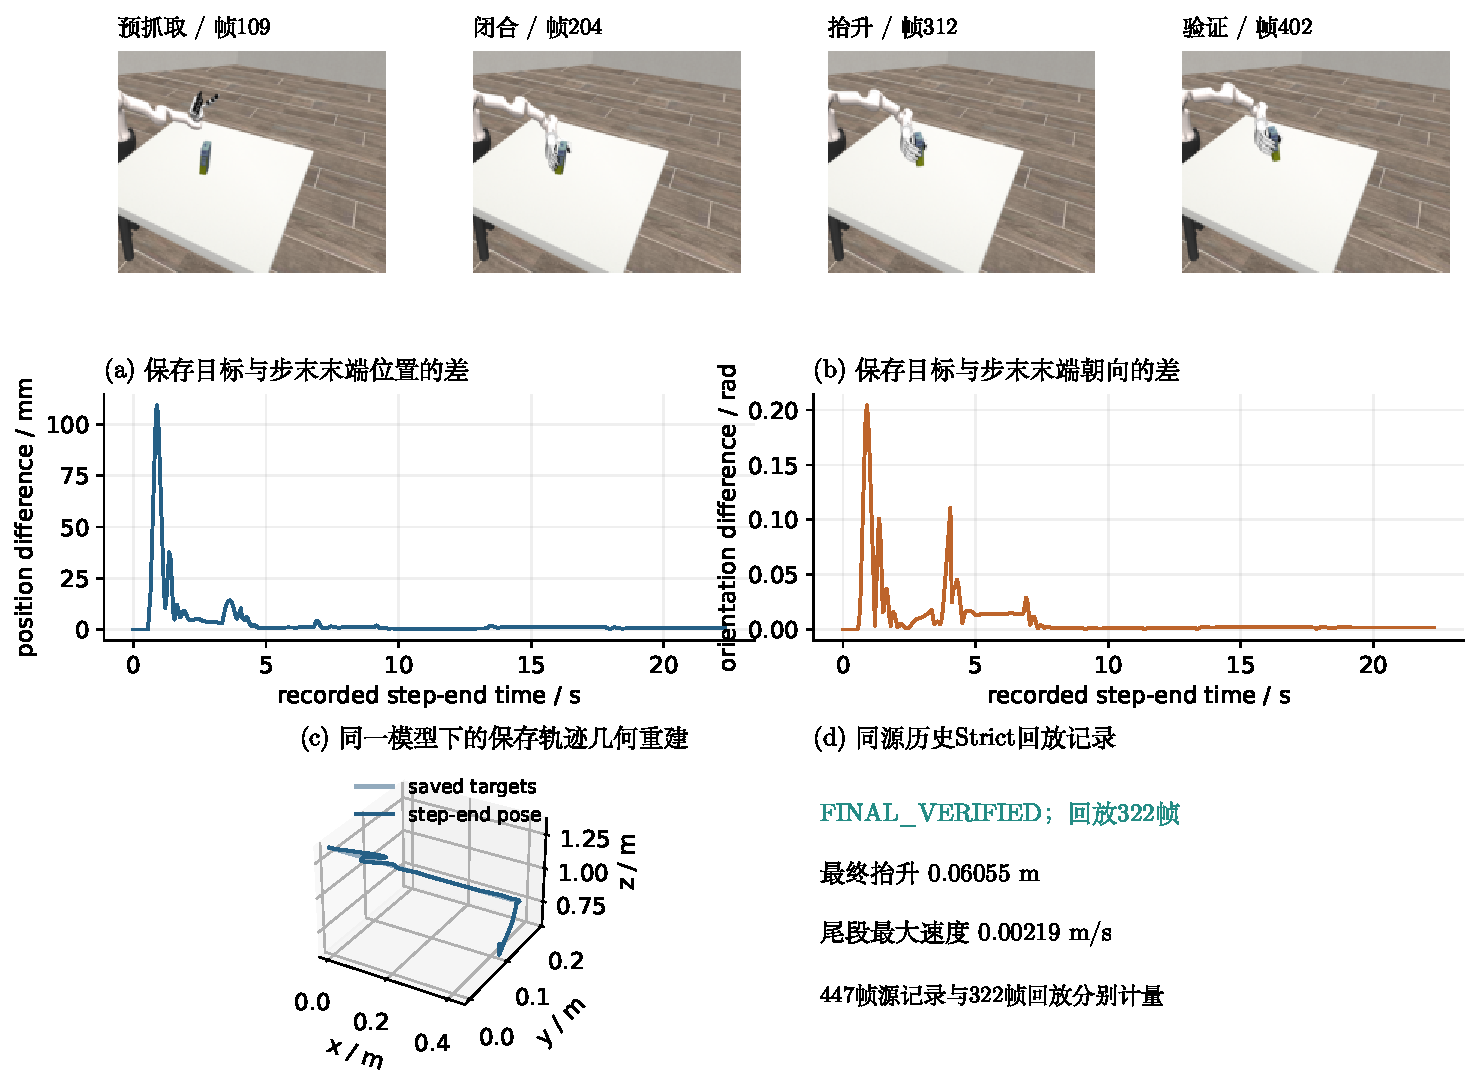
\includegraphics[width=0.97\textwidth]{figures/annotation_R2/recorded_tracking_strict.pdf}
  \caption{保存模型与关节状态的末端跟踪重建及同源历史Strict结果}
 \label{fig:ch03_strict_replay}
\end{figure}

图\ref{fig:ch03_recorded_trajectory}给出一条Sugar Box历史抬升记录中的命令与执行反馈。阶段边界直接取自保存的stage字段，三幅图共用记录时间轴。关节位置命令描述控制器要求，物体高度和接触数则反映实际执行过程：闭合与保持阶段建立接触，抬升阶段物体高度随之变化。将这些记录放在同一时间轴上，可以检查操作阶段与物体运动是否相衔接，并定位接触建立或丢失的时刻。该例用于展示历史执行过程，Strict质量仍按相应验证记录及其阈值判定。

\begin{figure}[htbp]
  \centering
  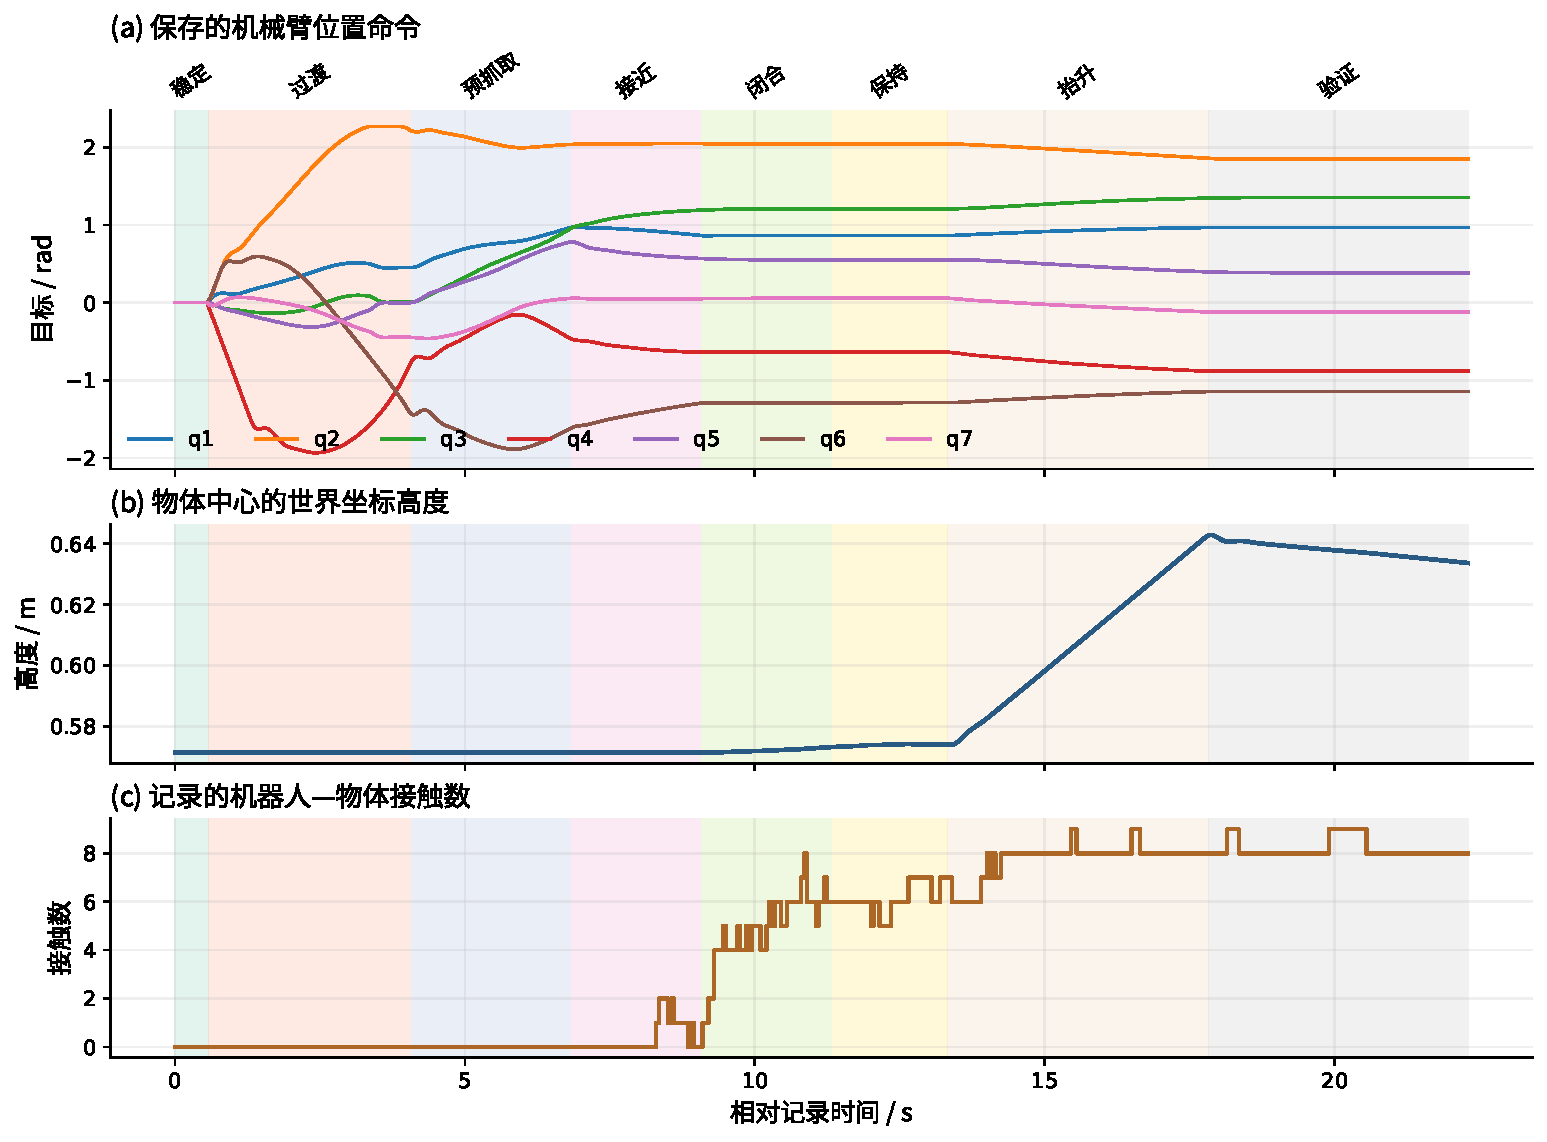
\includegraphics[width=0.96\textwidth]{figures/annotation_batch2/historical_lift_trajectory.pdf}
  \caption{Sugar Box历史抬升示教的位置命令、物体高度与接触反馈}
  \label{fig:ch03_recorded_trajectory}
\end{figure}

图\ref{fig:ch03_strict_replay}进一步利用另一条开发记录保存的模型快照与447帧关节状态，作静态正运动学重建。位置差为步末末端位置与同一行保存IK目标之差的范数，朝向差取四元数对应的最短旋转角；它们包含目标滤波、伺服和动力学跟踪影响，区别于IK求解器内部残差。关键阶段画面也仅恢复保存姿态。图中同源历史Strict文件登记322帧回放为FINAL\_VERIFIED，源序列与回放帧数分别标注，未在本次绘图中重新执行验证。

已有普通Replay接口主要检查控制序列能否回放，以及尾段任务成功比例。其成功条件要求最后一个尾段标记为成功，且尾段成功比例至少为0.8。该接口并未完整表达严格示教所需的稳定性条件，因此另外采用图\ref{fig:ch03_strict_replay}所示的Strict Replay。在对应仿真环境中重放实际低层控制序列后，Strict同时检查抬升、速度、角速度、皮肤接触和环境碰撞等指标，当前final配置见表\ref{tab:ch03_strict_thresholds}。

\begin{table}[htbp]
 \centering\small
 \caption{当前final配置的Strict Replay验收条件}
 \label{tab:ch03_strict_thresholds}
 \begin{tabular}{p{0.39\textwidth}p{0.17\textwidth}p{0.30\textwidth}}
 \hline
 指标 & 阈值 & 判定范围\\
 \hline
 最终及尾段最小抬升 & $\geq0.055$~m & 二者均需满足\\
 物体线速度 & $\leq0.10$~m/s & 尾段最大值\\
 物体角速度 & $\leq0.10$~rad/s & 尾段最大值\\
 皮肤接触、抓持比例 & 均$\geq0.80$ & 尾段统计\\
 机器人与桌面接触比例 & $\leq0$ & 尾段统计\\
 最大穿透 & $\leq0.003$~m & 尾段最大值\\
 验证尾段、额外保持 & 20步、12步 & 当前配置参数\\
 \hline
 \end{tabular}
\end{table}

Strict中的皮肤接触与抓持具有具体语义，不将任意机器人连杆碰撞当作有效指面抓持。全程最大穿透和尾段最大穿透虽然都被记录，实际最终布尔条件使用后者；若将全程记录量误写为硬门槛，就会改变原验证协议。最终及尾段最小抬升同时受限，也意味着物体曾短暂达到目标高度并不足够，尾段仍需满足要求。速度和角速度限制进一步区分持续承载与明显滑移、旋转等不稳定状态，桌面接触条件则避免利用环境支撑冒充稳定悬持。

验收状态由实际profile及布尔结果共同确定，final配置通过时记为FINAL\_VERIFIED，否则为FINAL\_REJECTED。生成过程中的某个变量即使名为strict\_execution，也不能替代该最终状态。类似地，物理执行返回success与严格回放通过是不同证据，候选档案、模板清单和示教导出需要保留验证层级。导出入口默认先进行final检查，诊断性允许未验证轨迹的开关不能作为正式质量保证。

轨迹重放还必须使用正确的动作语义。旧生成记录中的action可以是末端IK指令，ctrl则保存实际施加的机械臂七通道与手部六通道位置命令。二者均可能为十三维，但直接用前者替代后者会改变回放问题。记录器保存的关节状态、对象姿态和控制量有助于检查这种对应，完整时间关联则在第四章讨论。Strict通过只说明给定模型、初态、控制序列及阈值下的结果，不认证任意后续模型版本均能复现，也不把同一轨迹的后缀当成新的独立专家示教。

算法\ref{alg:grasp_demonstration_pipeline}归纳候选到示教的分层处理关系，各任务仍采用其专属执行与验证条件，不将这一归纳视为所有任务均调用同一实现。
\begin{algorithm}[H]
\small
\caption{抓取候选筛选与专家示教验证流程}\label{alg:grasp_demonstration_pipeline}
\KwIn{物体与资产版本、初始条件、候选来源及任务配置}
\KwOut{示教记录、任务结果及适用的验证状态}
利用已有候选来源获得几何候选，保留来源与评分\;
\ForEach{有限预算内的候选及局部腕姿编辑}{
将物体相对目标转换至机器人末端目标，补偿安装变换\;
求解预抓取与抓取目标IK，检查残差和关节条件\;
\If{未通过当前层的筛选}{登记失败类别，继续下一候选\;}
按任务配置构造分段目标并执行，记录状态、低层命令与结果\;
对要求独立Strict检查的轨迹，依据对应配置执行回放与联合检查\;
分别登记任务结果和验证状态，保留失败记录及来源\;
}
按任务专属条件整理专家示教，不以单目标可达替代完整执行检查\;
\end{algorithm}

\section{多任务专家示教生成}
\label{sec:multitask_demonstration}

多任务示教共享候选来源、控制序列、对象状态和阶段信息等记录合同，但采用不同控制逻辑。Lift提供基本抓持案例，其他任务依据操作目标构造后续过程，并以实际物体状态而非执行器目标判断结果。主要阶段见表\ref{tab:ch03_task_stages}。

Lift执行从稳定初态开始，经过过渡和预抓取接近，在close阶段逐步建立手部闭合命令，在hold阶段检查和维持接触，然后抬升并进入verify。接近阶段需要机械臂跟踪手部目标，接触阶段则要求驱动命令与物体几何形成有效加载；两者失败不能用同一几何指标解释。完整阶段记录让后续能够判断失败发生在物体接触之前还是加载之后，也为其他任务选择可用抓持前缀提供依据。

PickPlace以源抓持为基础，增加抬高避让、横向运输、下降、释放、撤离及任务验证。转移时既要保留物体初态与抓持目标的关系，也要考虑手部和桌面之间的几何余量。当前实现存在恢复已验证Lift终态并复用原前缀的路径，也存在从reset重新执行的选择。前者可以避免重复执行中的数值漂移，却不能被描述成整个拼接序列在该次运行中全部重新产生。对示教而言，前缀来源及衔接方式应明确保留，不能只凭拼接后数组长度判断物理连续性。

后续在线记录工作对原有前缀复用分支作了区分，重新执行时保留实际观测和控制，不将历史Lift触觉直接复制成新采集结果。这项修复说明示教生成与数据保存之间存在接口约束：任务控制完成和记录正确并不是同一个条件。本节只交代两种生成路径及其限制，完整模态关联与修复验收由第四章展开，不把修复后的合同回填为全部历史文件都已具备的属性。

\begin{table}[htbp]
 \centering\small
 \caption{五类任务的示教阶段与主要执行约束}
 \label{tab:ch03_task_stages}
 \begin{tabular}{p{0.15\textwidth}p{0.42\textwidth}p{0.29\textwidth}}
 \hline
 任务 & 主要阶段 & 执行重点\\
 \hline
 Lift & settle、transit、pregrasp、approach、close、hold、lift、verify & 接近跟踪、对向接触与抬升保持\\
 PickPlace & 抓持前缀、clear、transport、descend、release、retreat、task\_verify & 来源保持、安全下降及释放后目标状态\\
 Stack & 抓取、目标定位、运输下降、释放、稳定性评价 & 被操作物与支撑物关系\\
 Push & 接触接近、接触检测、反馈推动、目标评价 & 持续推动与物体实际位移\\
 NutAssembly & Bolt抓持、姿态伺服、平移、下降、装配评价 & 载荷保持、朝向与装配几何\\
 \hline
 \end{tabular}
\end{table}

Stack除被操作物之外还需要支撑物的状态。源抓持能够提供手与物体的相对关系，但堆叠目标必须根据支撑物位置、物体尺寸和下降范围进一步确定。任务后缀通过运输、下降和释放形成支撑关系，再检查物体是否稳定放置。并非每个物体都适合当前堆叠定义，因此已有批次先选取task-valid对象域。对这一筛选应保留来源，不能将限定物体域上的成功比例写成对任意物体的覆盖能力。

图\ref{fig:ch03_task_transfer}按各源序列保存的阶段选取中点画面。Lift展示抓持前缀与抬升，PickPlace展示抓持后的运输和释放；Stack所示记录从已有抓持状态后的运输阶段开始，支撑物贯穿下降和释放过程。推动与装配分别展示持续接触和抓持后姿态调整、下降的不同操作要求。

\begin{figure}[htbp]
  \centering
  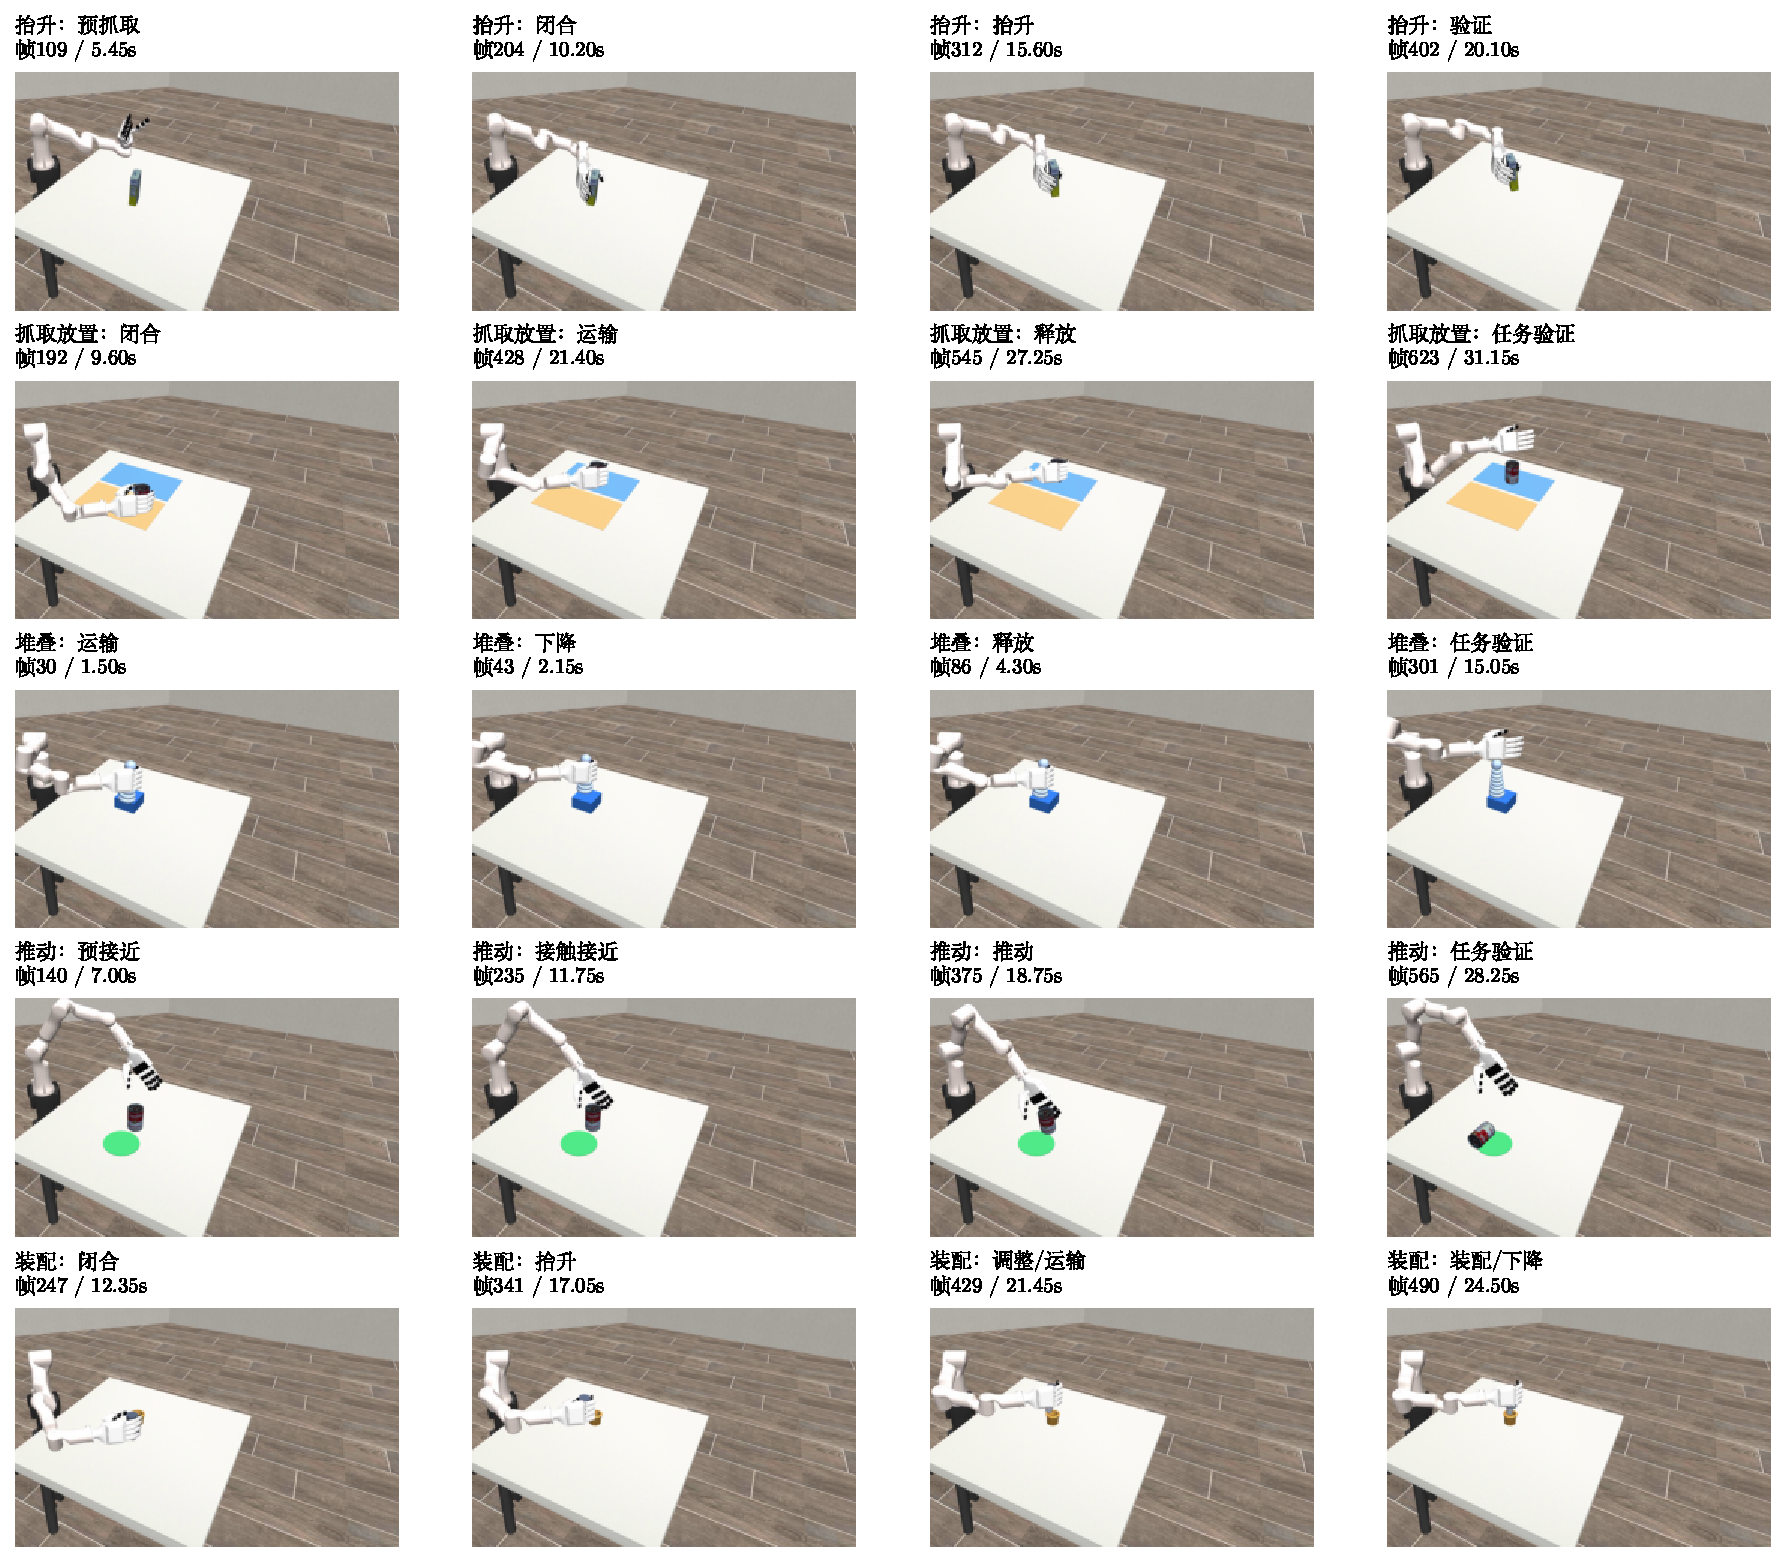
\includegraphics[width=0.97\textwidth]{figures/annotation_R2/five_task_phase_records.pdf}
  \caption{五类历史专家示教的实际阶段画面（按保存阶段中点选帧）}
 \label{fig:ch03_task_transfer}
\end{figure}

Push通过手掌或手指几何建立推动接触，并依据物体当前状态与目标位置的偏差反馈推进。其执行验证同时检查接触建立和物体实际位移，触觉用于描述推动阶段的接触响应。图\ref{fig:ch03_task_transfer}给出预接近、接触接近、推动及任务验证的历史画面，展示桌面支撑条件下的持续接触控制。

NutAssembly包含抓持Bolt、姿态伺服、平移、下降与装配结果评价。抓持阶段的细小偏差可能使物体倾斜，在后续下降前就丢失可用接触，因此不能把所有装配失败都归因于对孔精度。现有实现保留手部控制策略对承载过程的影响，也保留旧variant与后续几何版本不兼容的记录。局部成功可以用于分析某个控制条件是否值得保留，却不足以说明不同初态都能稳定装配，更不能把旧版本成功清单当成当前几何的最终验收。

上述专家示教通过候选、规划和任务反馈控制生成\cite{mandlekar2022demonstrations,mandlekar2023mimicgen}。每条轨迹随同保存任务条件、执行结果和验证状态，使后续使用者能够区分成功示例、失败示例与严格回放合格轨迹。第四章进一步讨论这些记录的时序配对、格式转换和来源追踪。

\section{抓取及示教质量实验}
\label{sec:grasp_quality_experiments}

本节依次考察候选路由能否提供可用模板、局部扰动示教是否满足Strict条件，以及执行失败发生在哪些阶段。表\ref{tab:ch03_historical_batches}先集中列明历史批量记录的来源与统计单位，再用具有源数组和验证文件的具体案例分析接触保持与轨迹质量。

Lift的100个对象标识中，98条由格点模板路由登记成功，2条由强化学习编辑路由登记成功，表明局部腕姿搜索是该批次主要的模板来源。PickPlace与Push分别登记100条SUCCESS，其缓存身份在表中单列；Stack在task-valid对象域中记录43条成功与5条失败；NutAssembly按variant记录100条成功。这些结果描述分级流程的产物覆盖，模块独立贡献则需要另设共同预算和初态的比较。

\begin{table}[htbp]
 \centering\small
 \caption{历史批量路由与任务记录及其统计限制}
 \label{tab:ch03_historical_batches}
 \begin{tabular}{p{0.16\textwidth}p{0.12\textwidth}p{0.30\textwidth}p{0.28\textwidth}}
 \hline
 任务或阶段 & 记录数 & 历史状态 & 解释限制\\
 \hline
 Lift候选路由 & 100 & 98 LATTICE\_SUCCESS，2 RL\_SUCCESS & 不是100条\newline\mbox{FINAL\_VERIFIED}\\
 PickPlace & 100 & 100 SUCCESS & 全部cached\\
 Stack & 48 & 43 SUCCESS，5 FAILED & 仅task-valid对象域\\
 Push & 100 & 100 SUCCESS & 98条cached\\
 NutAssembly & 100 & 100 SUCCESS & variant记录，非100个独立物体\\
 \hline
 \end{tabular}
\end{table}

上述批量表统一保留历史身份：Top100登记的18项源码Hash中，核对时12项相同、5项不同、1项对应文件缺失；cached表示复用结果，variant表示几何或配置变体，均以原记录单位计量。以下Sugar Box局部扰动与90次历史尝试另按各自来源和判据分析，避免以不同批次组成统一成功率。

局部扰动示教采用Sugar Box的10条既有记录。每份均有对应manifest，包含不同seed及不同NPZ Hash，源文件Hash与原审计登记一致，10份历史Strict结果均为FINAL\_VERIFIED。表\ref{tab:ch03_sugar_strict}列出其最终抬升和尾段角速度，展示严格通过并不只依赖数组中的成功标签。各记录使用同一物体和相近源抓取，历史审计记载不同初始位置的两两距离为0.707--2.828~mm，属于局部条件变化，不是大范围工作空间或跨物体泛化测试。

\begin{table}[htbp]
 \centering\small
 \caption{Sugar Box局部扰动示教的历史Strict结果}
 \label{tab:ch03_sugar_strict}
 \begin{tabular}{rrrrl}
 \hline
 序号 & seed & 最终抬升（m） & 尾段最大角速度（rad/s） & 验收状态\\
 \hline
 1 & 18011 & 0.06431 & 0.04049 & FINAL\_VERIFIED\\
 2 & 18012 & 0.06304 & 0.00324 & FINAL\_VERIFIED\\
 3 & 18013 & 0.06304 & 0.00303 & FINAL\_VERIFIED\\
 4 & 18014 & 0.06299 & 0.00311 & FINAL\_VERIFIED\\
 5 & 18015 & 0.06115 & 0.05234 & FINAL\_VERIFIED\\
 6 & 18016 & 0.06387 & 0.04748 & FINAL\_VERIFIED\\
 7 & 18017 & 0.06265 & 0.00602 & FINAL\_VERIFIED\\
 8 & 18018 & 0.06420 & 0.00428 & FINAL\_VERIFIED\\
 9 & 18019 & 0.06400 & 0.04943 & FINAL\_VERIFIED\\
 10 & 18020 & 0.06304 & 0.00346 & FINAL\_VERIFIED\\
 \hline
 \end{tabular}
\end{table}

10条序列均在源模板附近通过历史Strict条件，说明该抓取在所记录的小范围初态变化下能够保持承载与尾段稳定。该结果适用于同物体、相近源抓取的局部条件，评价重点是示教质量而非算法间排名。

\begin{table}[htbp]
 \centering\small
 \caption{历史90次扰动尝试的汇总分类}
 \label{tab:ch03_generation_failures}
 \begin{tabular}{lrp{0.51\textwidth}}
 \hline
 汇总类别 & 次数 & 统计解释\\
 \hline
 接受 & 46 & 历史生成汇总中的接受结果\\
 Strict不稳定 & 18 & 进入严格检查后未满足稳定条件\\
 Lift失败 & 26 & 未形成相应成功抬升轨迹\\
 \hline
 \end{tabular}
\end{table}

表\ref{tab:ch03_generation_failures}的历史报告按90次尝试登记46条接受、18条Strict不稳定和26条Lift失败。Lift失败对应未完成成功抬升，Strict不稳定则说明完成前序执行后仍可能在尾段速度、角速度或接触条件上不合格。两层淘汰分别对应承载建立和稳定示教的不同要求。该表为历史汇总证据；附加诊断可能重叠，且与前述局部示教存在来源重用，故保留原分母分别报告。

典型Lift案例的历史Strict结果中，最终抬升为0.0608926~m，尾段接触和抓持比例均为1，支持在该条件下持续承载的解释。NutAssembly则保留原始执行失败、降低抓点后仍失败、在降低抓点基础上保留hold抓持命令后单例成功的对照。该结果提示问题可能在装配之前的抓持保持阶段已经形成，而非只与末端对准有关；但它只是局部控制条件的对照，不能解释为跨seed稳定提升。图\ref{fig:ch03_examples}直接对照三条保存序列的物体高度、接触数和阶段。失败记录没有视频，图中使用其自身数组；不同记录长度与阶段进度分别呈现，便于检查抓持、运输和装配阶段的接触变化。

\begin{figure}[htbp]
\centering
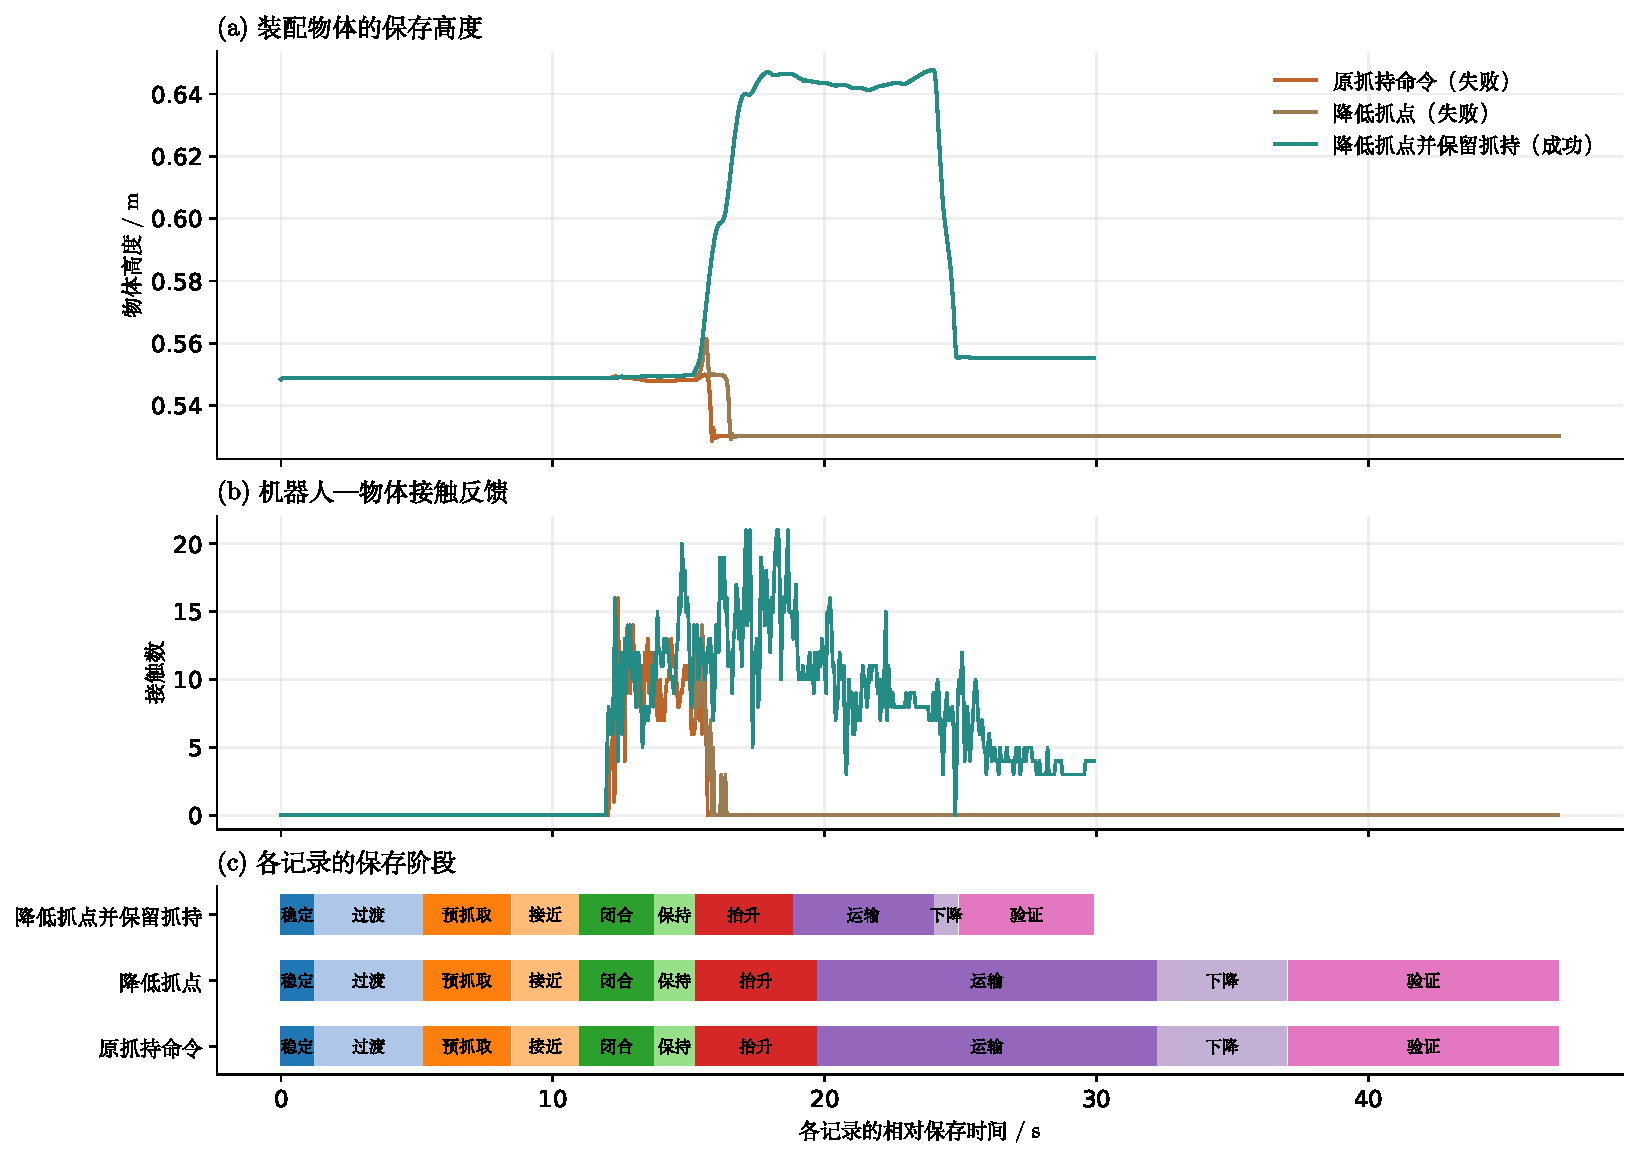
\includegraphics[width=0.97\textwidth]{figures/annotation_R2/assembly_failure_records.pdf}
\caption{装配历史成功与失败记录的物体高度、接触反馈和阶段对照}
\label{fig:ch03_examples}
\end{figure}

现有结果支持分层评价与任务专属控制的必要性，尚不支持模块间的公平优越性结论。缓存、variant和局部成功不合并为统一成功率；未定位原件的14物体与127物体批次不列入验证结果，也不用其他数量替代。

\section{本章小结}
\label{sec:grasp_demonstration_summary}

本章研究几何抓取候选到可执行专家示教的转换。候选表达限定手部控制变量，物理反馈检查抓持行为，可达性筛选与连续执行检验机器人运动条件，严格回放进一步检查轨迹质量。GraspQP官方指标被适配到六驱动手部代理，DexEvolve-style搜索与局部腕姿态扩展分别补充执行反馈和机器人可达性信息，条件性后续编辑用于处理部分尚未解决的案例。各环节在保留已有方法来源的基础上，分别处理抓持质量与机器人执行约束。

轨迹生成通过阶段目标、插值和控制器连续状态连接操作过程，Strict进一步区分任务成功与可用示教质量。已有批量记录、Sugar Box局部扰动Strict结果及典型任务对照提供了有限范围内的验证依据，但缓存记录、物体筛选域、历史版本及初态覆盖仍限制结论外推。五种任务共享记录合同，同时保留各自的接触、承载和目标评价逻辑。

执行成功的轨迹还需要转为语义明确的训练样本：策略在何时得到观测、下一步施加什么动作，以及这些记录来自哪次执行，都影响学习目标。下一章据此讨论多模态数据的组织、时序关联和质量审查。
